%growth rates not sig changed 
%v shear from thin dust layers are overwhelmed by 
\section{Discussion}\label{discussion}

\subsection{Generalization to locally polytropic disks}
We can extend the dusty/adiabatic gas correspondence to 
other fixed equations of state. As an example, consider the locally
polytropic disk 
\begin{align}
  P = K(r,z)\rhog^{\Gamma}, 
\end{align}
where $K$ is a prescribed function and $\Gamma$ is the constant
adiabatic index. Then eliminating $\tepsilon$ from the dust equation
\ref{dusteq} gives 
\begin{align}\label{poly_energy}
  \frac{D P}{D t} &= - \Gamma P\nabla\cdot\bm{v}  + P \bm{v}\cdot\nabla
  \ln{K} + \mathcal{C},\\
  \mathcal{C}& = \frac{\Gamma P}{\rhog}\nabla\cdot\left(\tepsilon\tstop\nabla
  P\right).
\end{align}
Thus the dusty gas behaves like a pure gas with adiabatic index
$\Gamma$. The entropy is given by 
\begin{align}
  \seff = \ln{\left[K^{1/\Gamma}(r,z)\left(1 - \tepsilon\right)\right]}.  
\end{align}
The results of \S\ref{iso_perfect}---\ref{dust_work} remain valid for the strictly 
polytropic disk with $K=$constant, while one sets $c_s^2\to K$ in
\S\ref{dusty_vsi_int}. 
%When $K$ is constant, the corresponding Solberg-Hoiland criteria for
%axisymmetric stability may be obtained from that in standard adiabatic 
%hydrodynamics \citep[e.g.][]{tassoul78} by
%using this definition of entropy in
%Eqs. \ref{dusty_solberg1}---\ref{dusty_solberg2}. 

\subsection{Implications for numerical simulations}
The dusty/adiabatic gas equivalence means that pure
gas dynamics codes can be applied to simulate locally
isothermal/polytropic dusty gas with minimal modification. In fact, no
modification is needed  
for strictly isothermal or polytropic gas perfectly-coupled to dust:  
the standard adiabatic energy equation substitutes for the dust continuity
equation. When $c_s$ or $K$ is not constant and/or $\tstop\neq0$ one
should add corresponding source terms in the energy equation
(e.g. Eq. \ref{poly_energy}). 
The source term associated with dust-gas drag, $\mathcal{C}$, is 
analogous to radiative diffusion \citep{price15}, which is also
featured in many hydrodynamics codes.      

\subsection{Dusty analogs of other gaseous instabilities}  

%gi
%rwi 

\subsubsection{Gravitational instability} %vertical structure 
The addition of dust enhances gravitational
instability (GI). This is because dust particles contribute to the
total disk mass but not thermal pressure, which effectively lowers the
disk temperature \citep[][]{thompson88,shi13}. For typical dust-loading 
$\epsilon, Z\ll1$, this effect is unimportant. However, if $\epsilon$ is
large (e.g. due to dust settling) then the effective temperature may 
be lowered to enable instability. 

As noted in \S\ref{loc_iso_eos}, dust settling causes the effective
temperature to \emph{increase} away from the midplane. This contrasts
to previous studies of GI in vertically stratified disks
 where the temperature decreases
from the midplane \citep[e.g.][]{mamat10, kim12,lin14c}. 
While we expect only the total surface density and
characteristic temperatures are relevant to stability  
\citep{toomre64}, a non-trivial effective vertical temperature
structure, induced by dust, may modify the vertical structure of 3D
waves and unstable modes. We will examine this linear problem in a following 
study.  



%see also
%\S\ref{loc_iso_eos}
%We thus expect the standard Toomre
%parameter to be modified to $Q = c_s\sqrt{1-\tepsilon}\Omega/\pi
%G\Sigma$. 

\subsubsection{Rossby wave instability}
The Rossby wave instability (RWI) is a non-axisymmetric, 2D shear
instability that operates in thin disks when it has radial structure
\citep{lovelace99,li00}. These studies consider adiabatic pure gas and 
show instability is possible if there is an extrema in the generalized
potential vorticity 
\begin{align}
 \mathcal{V} = \frac{\kappa^2}{2\Omega\Sigma}\mathcal{S}^{2/\gamma},  
\end{align} 
where $\mathcal{S} = \Pi/\Sigma^\gamma$. Here, $\Sigma$ is the total
surface density and $\Pi$ is the vertically integrated pressure. 

From the dusty/adiabatic gas equivalence, we deduce the corresponding
condition for RWI in a (locally isothermal or polytroipc) dusty gas is
also given by extrema in $\mathcal{V}$ with $\mathcal{S} = \exp{\left(\Gamma
S_\mathrm{eff}\right)}$ and $\tepsilon = \Sigma_\mathrm{d}/\Sigma$. Since
the effective entropy reflects the dust distribution, we expect that
RWI may also be triggered by extrema in the dust-to-gas ratio, e.g. 
narrow dust rings. This would lead to direction formation of dusty
vortices. 

%{\bf so may it's not vortex formation then dust-trapping. could just
%  form dusty vortices in one go}

%gap edges. thin dust rings. 

\subsection{New dust-drag
  instabilities}\label{dust_as_thermo} 

%{\bf vsi enabled by drag? slipping between dust and gas reduces
 % effective buoyancy}

As described in \S\ref{dust_work}, 
the physical cause of dust-drag instabilities is a phase lag between
the pressure and density response in a dusty gas\footnote{
In fact, we expect a phase difference between pressure and the total
density  whenever $\tstop\neq0$; not just $\tstop\OmK\ll 1$ as 
considered in this work. This is simply because of the finite
relaxation time required for dust to respond to gas, and vice versa. 
An effective energy equation in the form of Eq. \ref{eff_energy} can
still be obtained for general $\tstop$. The
heat flux $\bm{F}$ in the cooling function $\mathcal{C}$ is determined
through solution to the relative velocity $\Delta \bm{v} =
\bm{v}_\mathrm{d}-\bm{v}_\mathrm{g}$ \citep{youdin05a,laibe14}.  We
thus expect the `pressure-density lag' interpretation of dust-drag 
instabilities to be generally applicable.}. 
This may be used to re-interpret the streaming instability or to
understand other dusty instabilities. For example,
\cite{loren15,loren16} have recently discovered a new axisymmetric 
instability in their two-fluid numerical simulations of dusty
protoplanetary disks. They find it leads to the formation of
`toroidal vortices'. 

%give numerical example 
We have applied our one-fluid stability analysis to find unstable modes  
similar to that described by \cite{loren15}. We use the same
parameters reported by them as follows. 
%we set $p=q=0$, which eliminates VSI and minimizes streaming
%instabilities as there is no radial pressure gradient at the disk
%midplane.   
The total metalicity is $Z=0.01$ and the dust scale-height $H_\mathrm{d} =
0.4H_\mathrm{g}$, giving a maximum dust-to-gas ratio
$\mathrm{max}(\epsilon) = 0.025$. The midplane stopping time is 
$t_\mathrm{s0}=0.02\OmK^{-1}$. The gas disk parameters are $(p,q,
\hgas) =(-1.5, -1,0.05)$.  We set $k = \pi/H_\mathrm{d}$.      

Fig. \ref{compare_eigenvals_ts0d02} shows the unstable modes found for
this setup. We find the usual VSI modes, here with $\omega> 3\hgas\OmK,\, s<
0.2\hgas\OmK$. However, we also find modes with $\omega<s$. One of these,
marked by the blue asterisk, has 
frequency 
\begin{align*}
\sigma = (0.3631\ii - 0.1251)\hgas\OmK. 
\end{align*}
This growth rate corresponds to $8.8$ orbits, comparable to the $12$
orbits reported by \citeauthor{loren15}. We visualize this mode in
Fig. \ref{result2d_loren}. We find this mode 
persists when $q=0$, so it is not the VSI. 
Using Eq. \ref{streaming_dispersion} with the above parameters,  
we also estimate a much smaller growth 
rate for the streaming instability of 
$O(10^{-3}\hgas\OmK)$, We thus also rule out
SI, as did \citeauthor{loren15}. However, the mode disappears with $\tstop=0$, so it \emph{is}
associated with finite dust-gas drag. 

\begin{figure}
  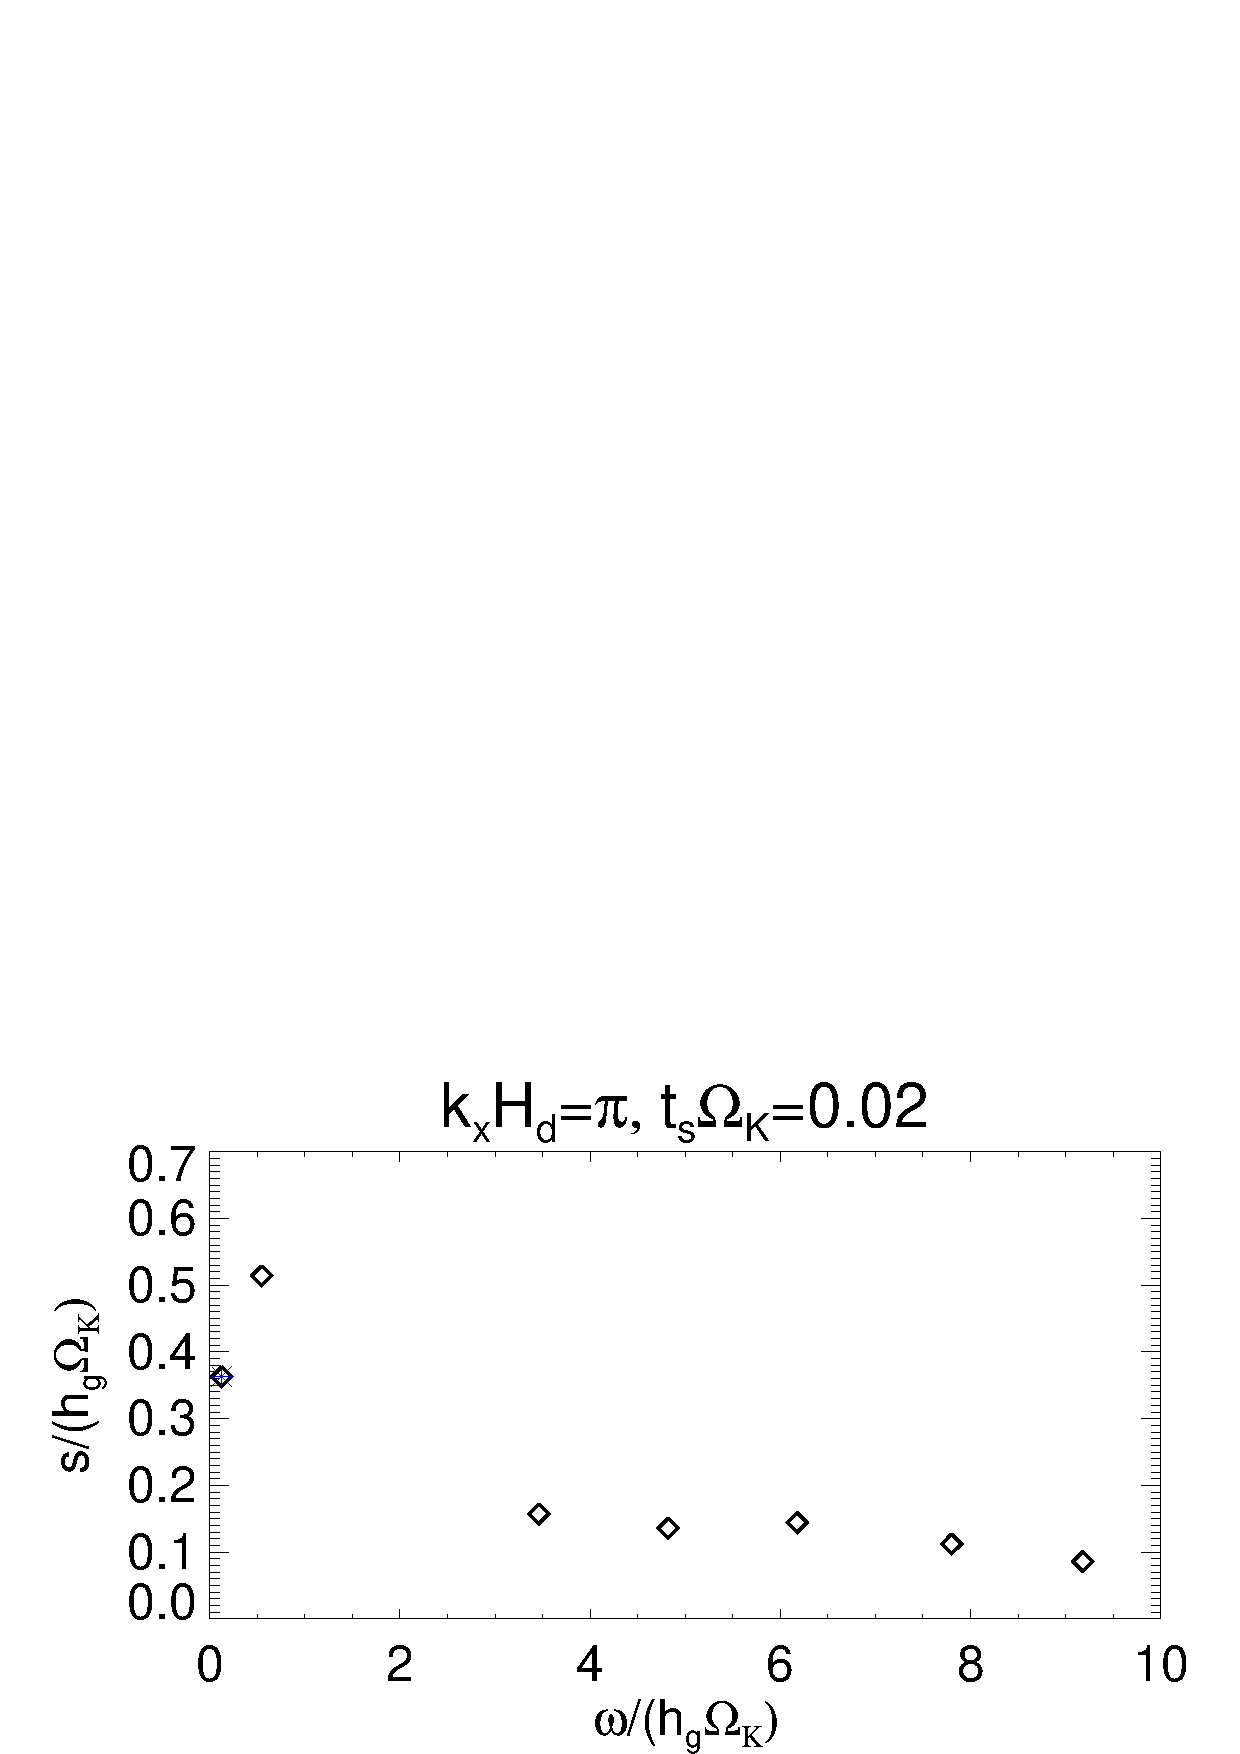
\includegraphics[width=\linewidth]{figures/compare_eigenvals_ts0d02}
  \caption{Unstable modes in a locally isothermal, dusty disk
    with stopping time  
    $\tstop=0.02\OmK^{-1}$. Modes with $\omega>3$ are due to
    VSI. The mode marked by the blue asterisk, visualized in
    Fig. \protect\ref{result2d_loren}
    , is associated with finite dust-gas
    drag. 
  }\label{compare_eigenvals_ts0d02}
\end{figure}


\begin{figure}
  \includegraphics[width=\linewidth]{figures/result2d_loren.ps}
  \caption{Visualization of the mode marked by the blue asterisk in
    Fig. \protect\ref{compare_eigenvals_ts0d02}. 
    This is a possible eigenmode of the dusty instability discovered by  
    \cite{loren15} in their numerical simulations. The instability growth timescale and 
    radial spacing of the `toroidal vortices' are similar to that 
    reported by \citeauthor{loren15}. This instability is driven by
    dust-gas drag. The color scale shows the 
    perturbed  
    dust-to-gas ratio, $\delta\epsilon$; and the arrows show
    $\sqrt{\rho}\left(\dd v_x, \dd v_z\right)$. 
  }\label{result2d_loren}
\end{figure}

One possible interpretation of this mode is `drag-driven VSI', to be 
compared with `cooling-driven VSI' studied by \cite{lin15}. In the
latter case, buoyancy forces are eliminated by fast
cooling, allowing vertical shear to destabilize the disk. Now, in an
isothermal dusty disk if $\tstop=0$ then mixture is 
effectively adiabatic: dust-induced buoyancy forces are
strongest. However, having $\tstop\neq0$ allow dust particles to slip
past the gas, reducing buoyancy. That is, dust-gas drag
provies an effective cooling. 

We stress that this example only serves to highlight
the possibility of new axisymmetric dust-drag instabilities in
stratified disks. A major caveat of the above result is that 
%the base state is not an exact equilibrium, because dust-settling would occur
%in practice. (
 the background dust settling timescale is comparable to the instability
growth timescale. It is essential to construct
exact equilibria for a meaningful stability analysis. We defer this
to future work.  

%also unclear what are "proper" vertical bc for dusty disks 

\section{Summary}\label{summary}
In this paper we describe the similarity between an isothermal 
dusty gas and an adiabatic, pure gas. The correspondence arises
because drag forces reduce the relative velocity between gas and
dust. In the limit of perfect dust-gas coupling, $\tstop \to 0$,  
 dust is entrained in 
the gas, and the dust-to-gas ratio $\rhod/\rhog$ is conserved
following the dusty flow. This is analogous to entropy being conserved
following a adiabatic, pure gas. 

For finite dust-gas drag, $\tstop\neq 0$, the dust content of a 
parcel of the mixture no longer conserved. The parcel 
can exchange dust particles with neighboring parcels owing 
to dust-gas relative drift. This is analogous to heat exchange between
a pure gas parcel and its surroundings. 

We explicitly show that for a locally isothermal, dusty gas that the 
evolutionary equation of  $\rhod/\rhog$ may be replaced by an 
effective energy equation. This leads to a 
natural definition of the effective entropy of isothermal dusty gas as  
\begin{align*}
  \seff  = \ln{\left(\frac{c_s^2\rhog}{\rhog+\rhod}\right)}.  
\end{align*}
%This allows us to define the buoyancy frequency of an isothermal 
%dusty gas. 
Finite dust-gas friction then appears as an energy
source term.  This analogy with standard 
hydrodynamics with cooling/heating allow us to obtain dusty analogs of gaseous
instabilities, and provide thermodynamical interpretations of  
dust-drag instabilities. 


We obtain the Solberg-Hoiland criteria for axisymmetric stability for
strictly isothermal, perfectly-coupled dusty gas.  
Applying this to typical protoplanetary disks, we find that 
the vertical shear associated with dust 
 layers \emph{cannot} lead to axisymmetric  
  instabilities, however thin the dust layer is.   
%This is consistent with the fact that only 
%\emph{non-axisymmetric} Kelvin-Helmholtz instabilities have been 
%observed in numerical simulations in the perfectly-coupled limit 
%\citep{chiang08,barranco09,lee10}. 
Instead, sharp radial  edges in the dust-to-gas ratio could destabilized the
disk, as these imply sharp gradients in the disk's effective entropy
profile. % {\bf presumably this limits how sharp dust rings can be} 

We  apply our thermodynamic framework to interpret
the streaming instability \citep[SI, ][]{youdin05a,jacquet11} and to generalize the vertical shear
instability \citep[VSI, ][]{nelson13,lin15} to dusty disks. We
explicitly show that the SI occurs because the evolution of gas
pressure lags behind  dust density; a general property of \emph{all}
instabilities driven by strong dust-gas drag. 
It takes a finite time for the gas to respond to
the dust motion. A lag implies a time interval when
gas pressure is still increasing while dust is already being expelled. 
The dusty gas then does positive work, which goes into amplifying
oscillation amplitudes. This interpretation is analogous to stellar pulsational
instabilities \citep{cox67}. 

For the VSI we find dust-loading is generally stabilizing. In our disk models 
dust-loading does not affect VSI growth rates significantly, but
meridional motions may be suppressed where the dust-induced
vertical buoyancy dominates over vertical shear, consistent with our
previous study \citep{lin15}.  

We also discuss future applications of our thermodynamic framework to 
study dusty protoplanetary disks. Because isothermal dusty gas has an
effective entropy, we suggest that purely hydrodynamic processes, such
as the Rossby Wave Instability \citep{li00} or the `Zombie Vortex
Instability' \citep{marcus15} could have dusty counter-parts.   
Furthermore, hydrodynamic instabilities driven by thermal cooling, such as VSI in
stably-stratified disks \citep{lin15} or the `Convective
Overstability' \citep{klahr14, lyra14},  may also find dusty analogs 
because finite dust-gas drag is equivalent to a heat sink/source. 

%In particular, we emphasize the 
%physical origin of any instability driven by strong dust-gas
%drag is a phase lag between the pressure and total density evolution
%of the dusty gas mixture. This leads to growing modes because 
%positive work is done during an oscillation cycle, provided by
%dust-gas drag, which is equivalent to a `heat' 
%source. 

%We demonstrate a potentially new dust-drag instability in
%stratified disks that may explain 
 
%We also applied
%our framework to find unstable modes in dusty, stratified disks
%similar to that reported recently by \cite{loren15}. 
